\apendice{Estudio experimental}



\section{Cuaderno de trabajo.}

En esta sección se describen los distintos pasos realizados a lo largo del proyecto con resultados tanto positivos como negativos.

\subsection{Redistribución de las imágenes}

En un principio, se intentó trabajar con las imágenes de CXT descargadas de internet tal y como venían en las carpetas distribuidas en ``\textit{train}'', ``val'' y ``test'' pero, se observó que los resultados que ofrecía no eran buenos, y, esto podía ser debido a una mala distribución en las imágenes. En la carpeta ``val'' venían únicamente 16 imágenes mientras que en la carpeta ``\textit{train}'' había un total de 5216 imágenes, por lo que existía mucho desequilibrio entre el conjunto de imágenes empleadas para el entrenamiento y el conjunto de imágenes empleadas para la validación. Los malos resultados pueden deberse a que una desigualdad entre el conjunto de imágenes de validación y el conjunto de imágenes de entrenamiento está relacionado con el sobreajuste y/o con una mala generalización de datos nuevos.

Por ello, se ha realizado una función en Python a partir de la cual, se distribuye de la manera deseada las imágenes en las distintas carpetas. La manera de distribuirlas ha sido un 64\% de las imágenes han sido destinadas a ``\textit{train}'', un 20\% para ``test'' y un 16\% a ``val''.

\subsection{Preprocesamiento de las imágenes y generación de iteradores}

Una vez obtenida la nueva carpeta con la nueva distribución de imágenes, se realizó otra función para generar iteradores con los conjuntos de entrenamiento, validación y prueba que se emplean para entrenar y evaluar el modelo.

Antes de generar los iteradores se tuvo que realizar un preprocesamiento de las imágenes para poder trabajar correctamente con ellas. Este preprocesamiento incluye un rescaldado de las imágenes, es decir la modificación del valor de los píxeles de [0,255] a [0,1] para normalizar las imágenes y un redimensionamiento de las imágenes a un tamaño de (150,150) o (340,340) según si se emplea la CNN propia o de AlexNet, ya que, las imágenes originales tenían cada una un tamaño distinto, y, para poder trabajar con ellas es necesario que todas tengan el mismo tamaño.

\subsection{Creación del modelo}

El siguiente paso, tras generar los iteradores, consiste en crear el modelo con el que se va a trabajar. Antes de llegar al modelo idóneo se deben probar numerosas combinaciones y numerosos parámetros. En este caso se partió del modelo más simple, compuesto por capas convolucionales, con las que se obtienen características importantes de las imágenes seguidas de capas de MaxPooling2D para reducir la dimensionalidad y sin capas ocultas. A partir de este modelo, se desarrollaron modelos más complejos, con capas ocultas.

A la hora de realizar el modelo más simple (figura \ref{fig:arquitectura_simple}), se probaron distintos valores de ``Dropout'' (0,1; 0,2; 0,3 y 0,5) y se llegó a la conclusión de que los mejores se resultados se obtenían con el 0,2 por lo que es el valor con el que se trabajó a posteriori.

\begin{figure}[h]
    \centering
    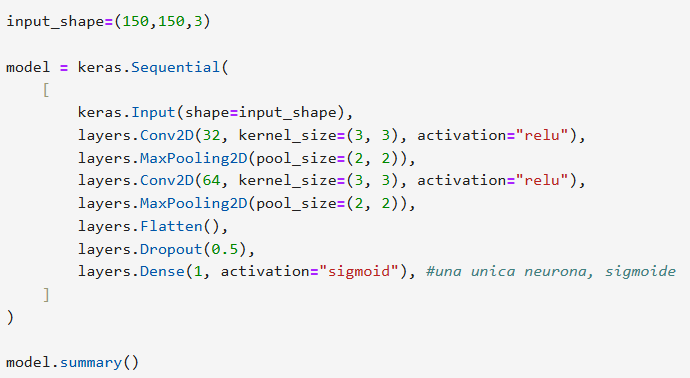
\includegraphics[width=0.99\textwidth]{img/arquitectura_simple.PNG}
    \caption{Modelo de arquitectura más simple. Fuente propia.}
    \label{fig:arquitectura_simple}
\end{figure}
\FloatBarrier

\subsection{Entrenamiento del modelo}

Tras haber creado el modelo, el entrenamiento se produce en dos pasos diferenciados. En primer lugar, se emplea ``model.compile'' para compilar el modelo, y, después ``model.fit'' para entrenarlo.

Al principio, se probó a ejecutar ``model.fit'' sin el parámetro de \textit{EarlyStopping} pero, tras la obtención de malos resultados se recomendó la investigación y el empleo de \textit{EarlyStopping} para una mejora de estos.

\subsection{Evaluación del modelo}

Aunque no se ve reflejado en este trabajo ya que no ha sido empleado finalmente, inicialmente se empleó la función de keras ``model.evaluate'' para la evaluación del modelo y obtención de métricas.

Pero, en este caso, se han calculado las métricas a mano y, se ha obtenido \textit{ytrain} (o las etiquetas de datos de entrenamiento) e \textit{ytest} (o las etiquetas reales de los datos de prueba) para obtener los resultados de las métricas y, a partir de estas métricas evaluar el modelo. Exceptuando la métrica \textit{loss}, la cuál sí se ha calculado a partir de ``\textit{model.evaluate}''.

\subsection{Creación de una función para el cálculo de métricas}

Para la obtención de las diversas métricas, se ha creado una función donde se calculan a mano (a partir de su fórmula) las diversas métricas que se emplean en este trabajo para su evaluación.

Las métricas se calculan a partir de los valores predichos por el modelo (y\_pred) y los valores con las etiquetas reales del conjunto de prueba (y\_test). Una vez se tienen estos dos valores, y, a partir de su matriz de confusión, se obtienen los verdaderos negativos, falsos positivos, falsos negativos y verdaderos positivos y, con esos valores ya se pueden calcular todas las métricas.

\subsection{Realización de diversas funciones para la comparación de diversos modelos, parámetros, etc.}

Una vez realizadas las primeras pruebas y entendidos los diversos pasos a seguir para el entrenamiento y la evaluación de un modelo, se procedió a buscar el mejor modelo para este caso concreto.

Para esto, se comenzó comparando distintos modelos de arquitectura, sin capa oculta, con una capa oculta y con dos capas ocultas. Se creó una función donde se incluyen estos tres modelos de forma que, para compararlos se accede directamente a esta función. 

A continuación, se creó otra función donde se incluye todo lo explicado previamente, es decir, la función donde se crean los iteradores de ``\textit{train}'', ``test'' y ``val'', el modelo con el que se va a trabajar (a partir de la función creada previamente), el entrenamiento del modelo, la evaluación del modelo y la obtención del \textit{dataframe} comparativo de cada modelo con sus correspondientes métricas. El objetivo de esta función fue comprar los distintos modelos y distintos \textit{batch size} para seleccionar el mejor. Para la realización de esta función se tuvieron que realizar algunos cambios en diversos parámetros hasta alcanzar unos resultados aceptables. Por ejemplo, se añadieron y quitaron parámetros de \textit{EarlyStopping}, se cambió la forma de obtención de las métricas en diversas ocasiones, etc.

Tras obtener el mejor modelo y su mejor \textit{batch size}, se creó otra función realizada de forma similar a la anterior para obtener el mejor valor de neuronas en la capa oculta. Al igual que en la anterior función, se llevaron a cabo diversos cambios antes de obtener los parámetros definitivos. En este caso, se tuvieron que probar también múltiples valores de neuronas para la capa o capas ocultas antes de obtener los ideales.

\subsection{Creación de dos CNN, una propia y otra obtenida a partir de la CNN AlexNet}

Debido a que, las métricas obtenidas en un inicio no eran buenas, aunque, los valores obtenidos durante el entrenamiento sí lo eran, además de probar y cambiar varios parámetros hasta encontrar el error, también se realizó un nuevo modelo de CNN, basado en la CNN de AlexNet.

En un principio, esta CNN era solo para comprobar donde estaba el error, pero, finalmente y, tras solucionar el problema de los malos resultados obtenidos en las métricas, se decidió mantener esta CNN para compararla con la CNN creada inicialmente y quedarse con aquella con la que se obtuvieran mejores resultados.

Por lo tanto, a la hora de comparar la mejor arquitectura y el mejor \textit{batch size}, se hizo tanto para la CNN propia como para la CNN basada en AlexNet.


\subsection{Obtención del \textit{dataframe} con las distintas métricas para cada modelo}

El objetivo de todo este proceso consiste en la obtención de un \textit{dataframe} donde se puedan ver y comparar las diversas métricas obtenidas para distintos modelos de red neuronal (con distinta CNN, arquitectura, parámetros, etc.).

Para la obtención de estos \textit{dataframes}, surgieron algunos problemas iniciales ya que, en un principio se imprimía el \textit{dataframe} original, pero, se llegó a la conclusión de que su tamaño era demasiado grande y no se podía mostrar bien en la \textit{memoria} por lo que, se decidió realizar algunos cambios tales como el redondeo a dos decimales de los números, la eliminación del índice o quitar los decimales de números enteros.

Inicialmente tampoco se guardaban estos \textit{dataframes} en ningún sitio, únicamente se imprimían por pantalla en el notebook correspondiente pero, esto se modificó para ser guaradados en formato csv dentro de la carpeta ``Resultados''.

\subsection{Matriz de confusión para la comparación de modelos}

También se ha una función para la obtención de la matriz de confusión del modelo más simple y del modelo final obtenido.

De esta forma se puede comprobar de una forma más visual la mejora de uno respecto al otro.

Para la realización de dichas matrices, es necesario guardar previamente los modelos creados tras cada entrenamiento en las diferentes funciones. De forma que, cuando se desee realizar la matriz de confusión para un modelo en concreto, bastará con cargar dicho modelo. Aunque, cabe mencionar que, inicialmente esto no se hizo así. Al principio, se copiaba y pegaba el modelo para el que se iba a realizar su matriz de confusión y se entrenaba de nuevo. Pero, se comprobó que de esta forma la matriz de confusión obtenida no estaba asociada al 100\% con los resultados de ese modelo obtenidos previamente ya que, debido a la aleatorización explicada en el apartado de \textit{Resultados} de la memoria, cada vez que se entrena el modelo, este puede variar sutilmente. Por lo que, se decidió modificar el código realizado y guardar todos los modelos entrenados para poder ser reutilizados posteriormente dentro de la carpeta ``Modelos''.

\subsection{Gráfica para ver el rendimiento del modelo en el entrenamiento y la validación}

En la creación de las funciones para la obtención de tablas comparativas con diferentes parámetros o arquitecturas, se guardan en un csv los resultados (o métricas) obtenidos en cada iteración para el entrenamiento y la validación dentro de la carpeta ``Historicos''. 

Posteriormente se crea una función para la obtención de una gráfica donde se visualiza el rendimiento del modelo a lo largo de las épocas con la métrica ``\textit{loss}'' o ``auc'' tanto para el entrenamiento como para la validación.

Gracias a esto, se puede observar de una forma más visual si los datos están entrenando correctamente, si existe algún tipo de sobreajuste, subajuste, etc.

\subsection{Se añaden todas las funciones en un archivo.py para ser ejecutadas en otro \textit{notebook}}

Una vez creadas todas funciones necesarias para la realización de este trabajo, se han copiado en un archivo.py para, posteriormente ser ejecutadas en un nuevo \textit{notebook}.

\section{Configuración y parametrización de las técnicas.}

Algunos de los parámetros, hiperparámetros y funciones o clases con una mayor relevancia en este trabajo son:

\begin{itemize}
    \item \textbf{\textit{batch size}}: el tamaño de lote o \textit{batch size}, se explica de forma más extensa en el apartado de ``\textit{Conceptos teóricos}'' de la memoria pero, resumiendo, corresponde con el número de muestras de entrenamiento que se propagarán a través de la red ~\cite{stackbatch24}.
    \item \textbf{\textit{epochs}}: el número de épocas corresponde con las iteraciones que se realizan sobre el conjunto de datos con un determinado \textit{batch size} ~\cite{diego23}. En este caso, se ha empleado un valor de 20 ya que, se trabaja a nivel de CPU (con el ordenador personal) y no GPU (con un supercomputador). Aumentar el número de épocas requeriría más recursos computacionales y tiempo de procesamiento, lo que podría afectar negativamente al rendimiento del ordenador y ralentizar significativamente el proceso de entrenamiento.
    \item \textbf{\textit{class\_mode}}: empleado a la hora de crear cada uno de los iteradores para el entrenamiento y la evaluación del modelo. En este caso se ha empleado el modo 'binary' ya que se trata de una clasificación binaria al haber solo dos clases ``NORMAL'' y ``PNEUMONIA''.
    \item \textbf{\textit{filters}}: se emplea en la clase Conv2D. Es un número entero que determina el número de filtros que tendrá la capa. Generalmente el valor aumenta capa tras capa \cite{kerasconv2d24, diego23}.
    \item \textbf{\textit{kernel\_size}}: se emplea en la clase Conv2D. Número entero o tupla de dos que determina el tamaño de la ventana de convolución o filtro \cite{kerasconv2d24}.
    \item \textbf{\textit{strides}}: se explica de forma más extensa en el apartado de ``\textit{Conceptos teóricos}'' de la memoria pero, resumiendo, corresponde con un número entero o tupla de dos que se emplea en la clase Conv2D y determina el número de columnas y de filas que se desplaza el kernal en cada operación de la convolución\\ \cite{kerasconv2d24, diego23}.
    \item \textbf{\textit{padding}}: se explica de forma más extensa en el apartado de ``\textit{Conceptos teóricos}'' de la memoria, pero, resumiendo, corresponde con un valor tipo \textit{string} que se emplea en la clase Conv2D y afecta a la dimensión de salida de la capa de convolución. Sus dos valores válidos son ``\textit{valid}'' y ``\textit{same}''. Donde ``\textit{valid}'' significa que la dimensión de salida es menor que la de la entrada y ``same'' significa que la longitud de salida es la misma que la longitud de entrada \cite{stackoverflowpadding24}.
    \item \textbf{\textit{pool\_size}}:  Número entero o tupla de dos que se emplea para reducir la dimensionalidad espacial.  En el caso de introducir un número entero, significa que el valor es el mismo para filas y columnas, sin embargo, si se introduce una tupla, el número de filas y columnas puede ser distinto.
    
    Representa el valor máximo de la ventana de entrada sobre el que se va a aplicar MaxPooling2D para realizar un submuestreo de los datos y quedarse con aquellas características más importantes reduciendo la carga computacional y evitando un posible sobreajuste \cite{kerasMaxPool24, diego23}. 
    \item \textbf{\textit{activation}}: a la hora de configurar el modelo, para la capa densa se debe configurar el parámetro \textit{activation}=``sigmoid'' debido a que se trata de un modelo de clasificación binaria y la función sigmoidea siempre devuelve un valor entre 0 y 1 ~\cite{kerassigmoid24}. Donde 0 se corresponde con ``NORMAL'' y 1 con ``PNEUMONIA''.
    \item \textbf{\textit{Dropout}}: ayuda a evitar el sobreajuste ~\cite{kerasdropout24}. En este caso, se han probado diversos valores tales como 0,1; 0,2; 0,3 y 0,5 y se ha determinado que los mejores resultados se obtenían con el 0,2 por lo tanto, es el que se ha empleado.
    \item \textbf{\textit{loss}}: se emplea en \textit{model.compile}, permite configurar el constructor según el argumento que se pase ~\cite{keraslosses24}. En este caso, se ha empleado como argumento la clase \textit{BinaryCrossentropy} ya que, se está trabajando con una clasificación binaria. \textit{BinaryCrossentropy} calcula la pérdida de entropía cruzada entre etiquetas verdaderas y etiquetas predichas ~\cite{kerasbinary24}.
    \item \textbf{\textit{optimizer}}: se trata de un argumento necesario para compilar un modelo Keras ~\cite{kerasOptimizers24}. En este caso, se ha empleado el algoritmo ``adam'', el cual adapta la tasa de aprendizaje para cada parámetro utilizando promedios móviles exponenciales de los gradientes y los cuadrados de los gradientes ~\cite{kerasAdán24}. En este caso, debido a que no se ha indicado ningún valor para \textit{learning rate} concreto, se asume que, se está empleando un \textit{learning\_rate}=0.001 que, es su valor por defecto.
    \item \textbf{\textit{EarlyStopping}}: es una clase la cual se explica extensamente en el apartado de ``\textit{Conceptos teóricos}'' de la memoria pero, resumiendo, su objetivo consiste en dejar de entrenar cuando una métrica monitoreada deja de mejorar ~\cite{kerasearly24}. Esta clase, incluye una serie de argumentos de los cuales, algunos se han incluido en este trabajo y se van a ver a continuación.
    \item \textbf{\textit{monitor}}: argumento de \textit{EarlyStopping} que indica la cantidad que se monitorea ~\cite{kerasearly24}. En este caso se ha empleado ``val\_auc'' ya que es una de las métricas más relevantes para este trabajo.
    \item \textbf{\textit{patience}}: argumento de \textit{EarlyStopping} el cual indica después de cuantas épocas se ha de detener el entrenamiento en caso de que no mejore ~\cite{kerasearly24}. En este caso se ha asignado a 10 épocas.
    \item \textbf{\textit{restore\_best\_weights}}: argumento de \textit{EarlyStopping} con el cual el modelo finaliza con los mejores pesos encontrados durante el entrenamiento al haberlo asignado a ``\textit{True}''. En caso de ser asignado a ``\textit{False}'', el modelo finalizaría con los pesos de la última época entrenada antes de la detención ~\cite{kerasearly24}.

    
\end{itemize}




